\scanpage{4}

\uline{(Structure modérée sur un espace)}

§ 1) $X$ ensemble \deleted{topologique}

$\deleted{\unsure{\mathcal E}}\inserted{F}$ ens. de parties de $X$, satisfaisant les conditions

b) $\deleted{\unsure{\mathcal E}}\inserted{F}$ stable pr réunions \unsure{finie|finies}

b') $\deleted{\unsure{\mathcal E}}\inserted{F}$ stable pr intersections finies

\unsure{a)} $F$ stable pr passage au complémentaire

\figure{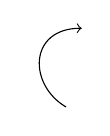
\begin{tikzpicture}[x=0.4cm,y=0.4cm]\draw[->] (0,0) .. controls (-1.2,0.7) and (-1.2,2.5) .. (0.5,2.5);\end{tikzpicture}}

Si $\deleted{\unsure{F}}\mathcal A_F$ est l'ens des fonctions sur $X$, à valeurs dans $\mathbb{Z}$ (disons), ne prenant qu'un nb fini de valeurs, et telles que $\forall n\in \mathbb{Z}$, on a $f^{-1}(\{n\})\in F$, \deleted{alors de sorte que} \inserted{alors} a) équivaut à la condition

\margin{\unsure{moyennant b)} $\mathcal A_F$ \unsure{contient l'ens des constantes}}

a') $\forall A\in F$, la fonction caractéristique $\varphi_A$ de $A$ est $\in\mathcal A_F$

et par suite \inserted{moyennant a)} la donnée de $F$ équivaut à celle de la partie $\mathcal A_F\subset \mathbb{Z}^X$. Ceci dit, \deleted{\unsure{les}} moyennant a) les conditions b) et b') sont équivalentes, et équivalent à la suivante :

b'') $\mathcal A_F$ est stable par produits finis

\deleted{\unsure{b''')} $\mathcal A_F$ est \unsure{\(\ne\varnothing\)} et stable pr \unsure{\(+\)}}

et alors $\mathcal A_F$ est \deleted{\unsure{aussi}} \inserted{même} stable pr sommes finies, et pr \unsure{l'inv. des signes} par $f\mapsto-f$, donc c'est un sous-anneau unitaire de $X^\mathbb{Z}$. Plus généralement, si $\Lambda$ est un anneau \deleted{\unsure{$\ne0$}} \inserted{non nul}, on peut remplacer dans tout ceci \inserted{$\mathbb{Z}$ par $\Lambda$, et} $\mathbb{Z}^X$ par $\unsure{K^X|\Lambda^X}$ : Moyennant a) et b) $\mathcal A_F$ est une sous-$\Lambda$-algèbre de $\deleted{\unsure{\mathcal A}}\Lambda^X$. Soit $\operatorname{Et}(X,\Lambda)$ l'alg. des fonctions ``\uline{étagées}'' sur $X$ à valeurs dans $\Lambda$ (i.e. ne prenant qu'un \deleted{\unsure{seul}} \inserted{nb fini de} valeurs). Alors $F$ est connu quand on connaît la sous-algèbre $\mathcal A_F$ de $\operatorname{Et}(X,\Lambda)$. Lorsque $\Lambda$ est intègre de corps

\mspage{5}
